\hypertarget{iv-linear-scalable-transformer-model}{%
\subsection{IV Linear Scalable Transformer
model}\label{iv-linear-scalable-transformer-model}}

As stated earlier, the proposed model proposes the replacement of the
scaled dot-product attention from original Transformer architecture by a
kernelized attention with relative positional encoding

The proposed model replaces the scaled-dot-product-attention by a
kernelized attention with RPE. Following the observations of
\href{https://arxiv.org/abs/1803.02155}{Shaw et al.~(2018)} that
cumulating absolute positional encoding with relative positional
encoding yield no benefits, the positional encoding is also removed -
althought for some specific applications it might be beneficial to
maintain it. The algorithm used to calculate each term is chosen
dynamically to occupy the least memory depending on the sequence lengths
and embedding dimensions - as memory usage is easier to evaluate
precisely than execution time.

In this work we have chosen the following formulation, with
\(\phi(x) = elu(x) + 1\).

\[A = \frac{\left( \phi(Q) \times \phi(K^T) + S^{rel} \right)}{\sum_j \left( \phi(Q) \times \phi(K^T) + S^{rel} \right)} \times V\]

This is essentially a combination of two terms: the kernelized attention
proposed by \href{https://arxiv.org/abs/2006.16236}{Katharopoulos et
al.~(2020)}, and the relative positional encoding proposed by
\href{https://arxiv.org/abs/1803.02155}{Shaw et al.~(2018)}. The left
term is the score matrix of shape \((L_Q, L_K)\), with a denominator
which scales all rows so that they sum to 1. For the sake of the
implementation, the multiplication must be distributed as:

\[A = \frac{\left( \phi(Q) \times \phi(K^T) \times V \right) + \left( S^{rel} \times V\right)}{\sum_j \left( \phi(Q) \times \phi(K^T) \right) + \sum_j \left( S^{rel} \right)}\]

The denominator can be easily calculated by applying the (naive or
linear complexity) algorithms with V replaced by a matrix of shape
\((L_K, 1)\) full of 1.

For each case (masked/bidirectional) the algorithm is chosen between
naive and linear complexity to occupy the least memory.

\begin{itemize}
\tightlist
\item
  for the masked \(Q \times K^T \times V\) term, the memory occupied by
  the naive algorithm is \(L_QL_K\) while the linear complexity
  algorithm occupies \(d^2 \times max(L_Q, L_K)\)
\item
  for the bidirectional \(Q \times K^T \times V\) term, the memory
  occupied by the naive algorithm is \(L_QL_K\) while the linear
  complexity algorithm occupies \(d^2\)
\item
  for the \(S_{rel} \times V\) term (masked and bidirectional), the
  memory occupied by the naive algorithm is \(L_QL_K\) while the linear
  complexity algorithm occupies \(L_Q \times (2k+1 + 4)\)
\end{itemize}

\hypertarget{v-results}{%
\subsection{V results}\label{v-results}}

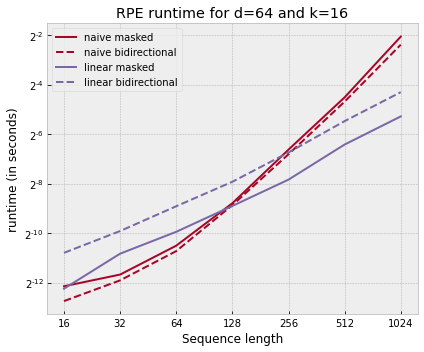
\includegraphics{images/timings/runtimes_RPE.png}

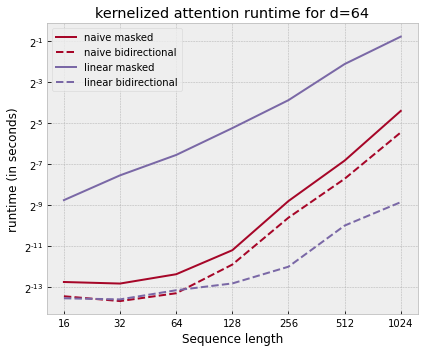
\includegraphics{images/timings/runtimes_KA.png}

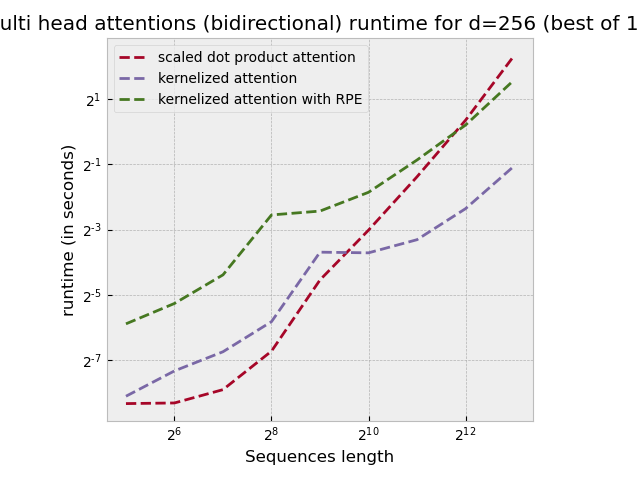
\includegraphics{images/timings/runtimes_MHA.png}

\hypertarget{conclusion}{%
\subsection{Conclusion}\label{conclusion}}

In the present work an easily implemented algorithm to compute
\href{https://arxiv.org/abs/1803.02155}{Shaw et al.~(2018)}'s relative
positional embedding with linear complexity has been presented. An
implementation of \href{https://arxiv.org/abs/2009.14794}{Choromanski et
al.~(2020)}'s prefix sum algorithm that doesn't requires custom CUDA
code (while maintaining linear complexity) was also presented.

These two elements allowed to define a kernelized attention function
with relative positional encoding, that can be computed with linear
complexity with regards to sequence length. The proposed model presents
linear scalability with sequence length, can be implemented out of the
boxe in neural network framework, and is adapted to sequence to sequence
problems instead of being restricted to encoders only models.
